% https://tex.stackexchange.com/a/159294/316176
\newcommand{\rulesep}{\unskip\ \vrule\ }

\begin{figure*}
  \centering
  \begin{subfigure}[b]{0.33\textwidth}
    \centering
    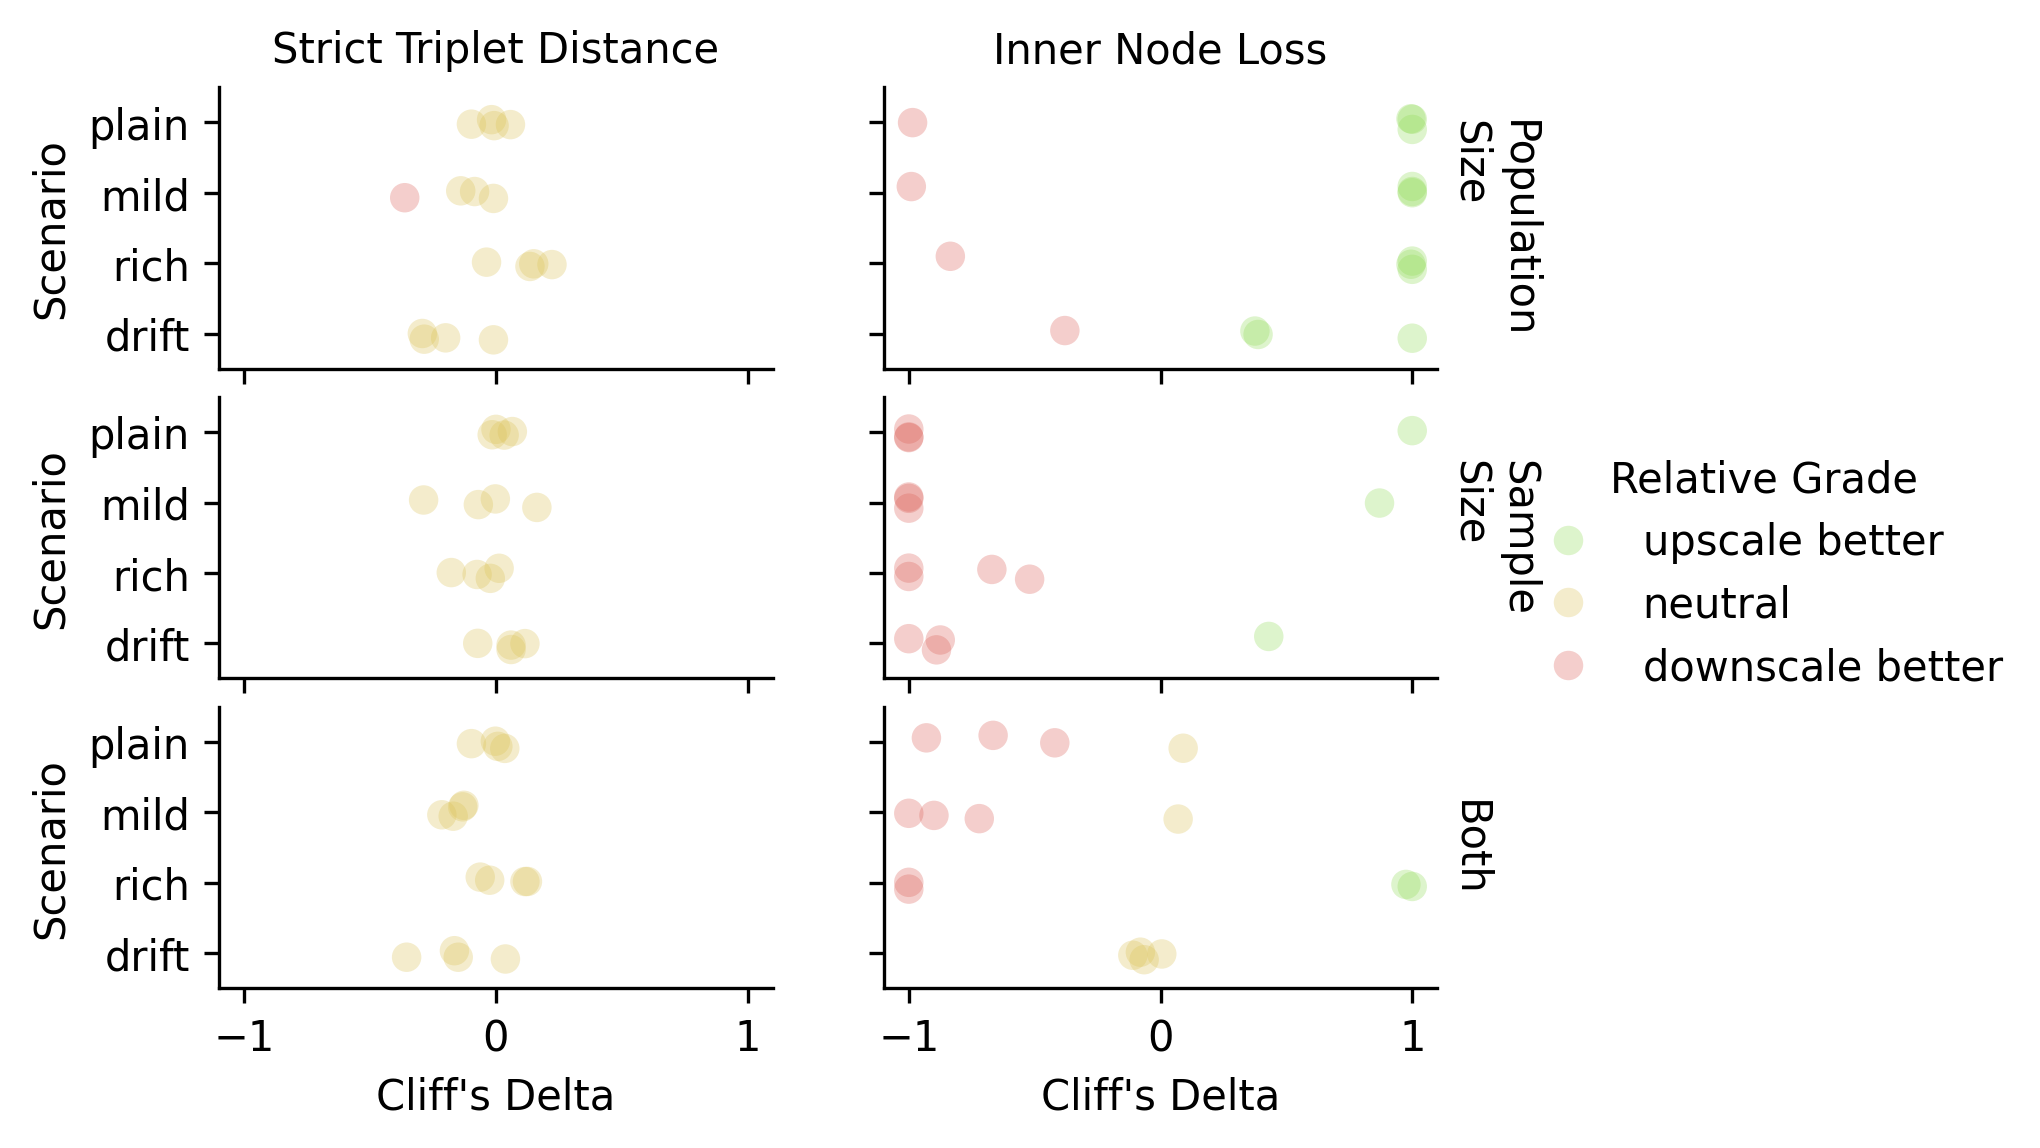
\includegraphics[height=1.7in,trim={0 0 5cm 0},clip]{binder/binder/dsamp-popsize-scale/teeplots/col=metric+hue=relative-grade+kind=strip+policy=tilted+row=scaling-factor+viz=catplot+x=cliff-s-delta+y=scenario+ext=}
    \caption{tilted retention policy (surface)}
  \end{subfigure}%
  \rulesep %
  \begin{subfigure}[b]{0.26\textwidth}
    \centering
    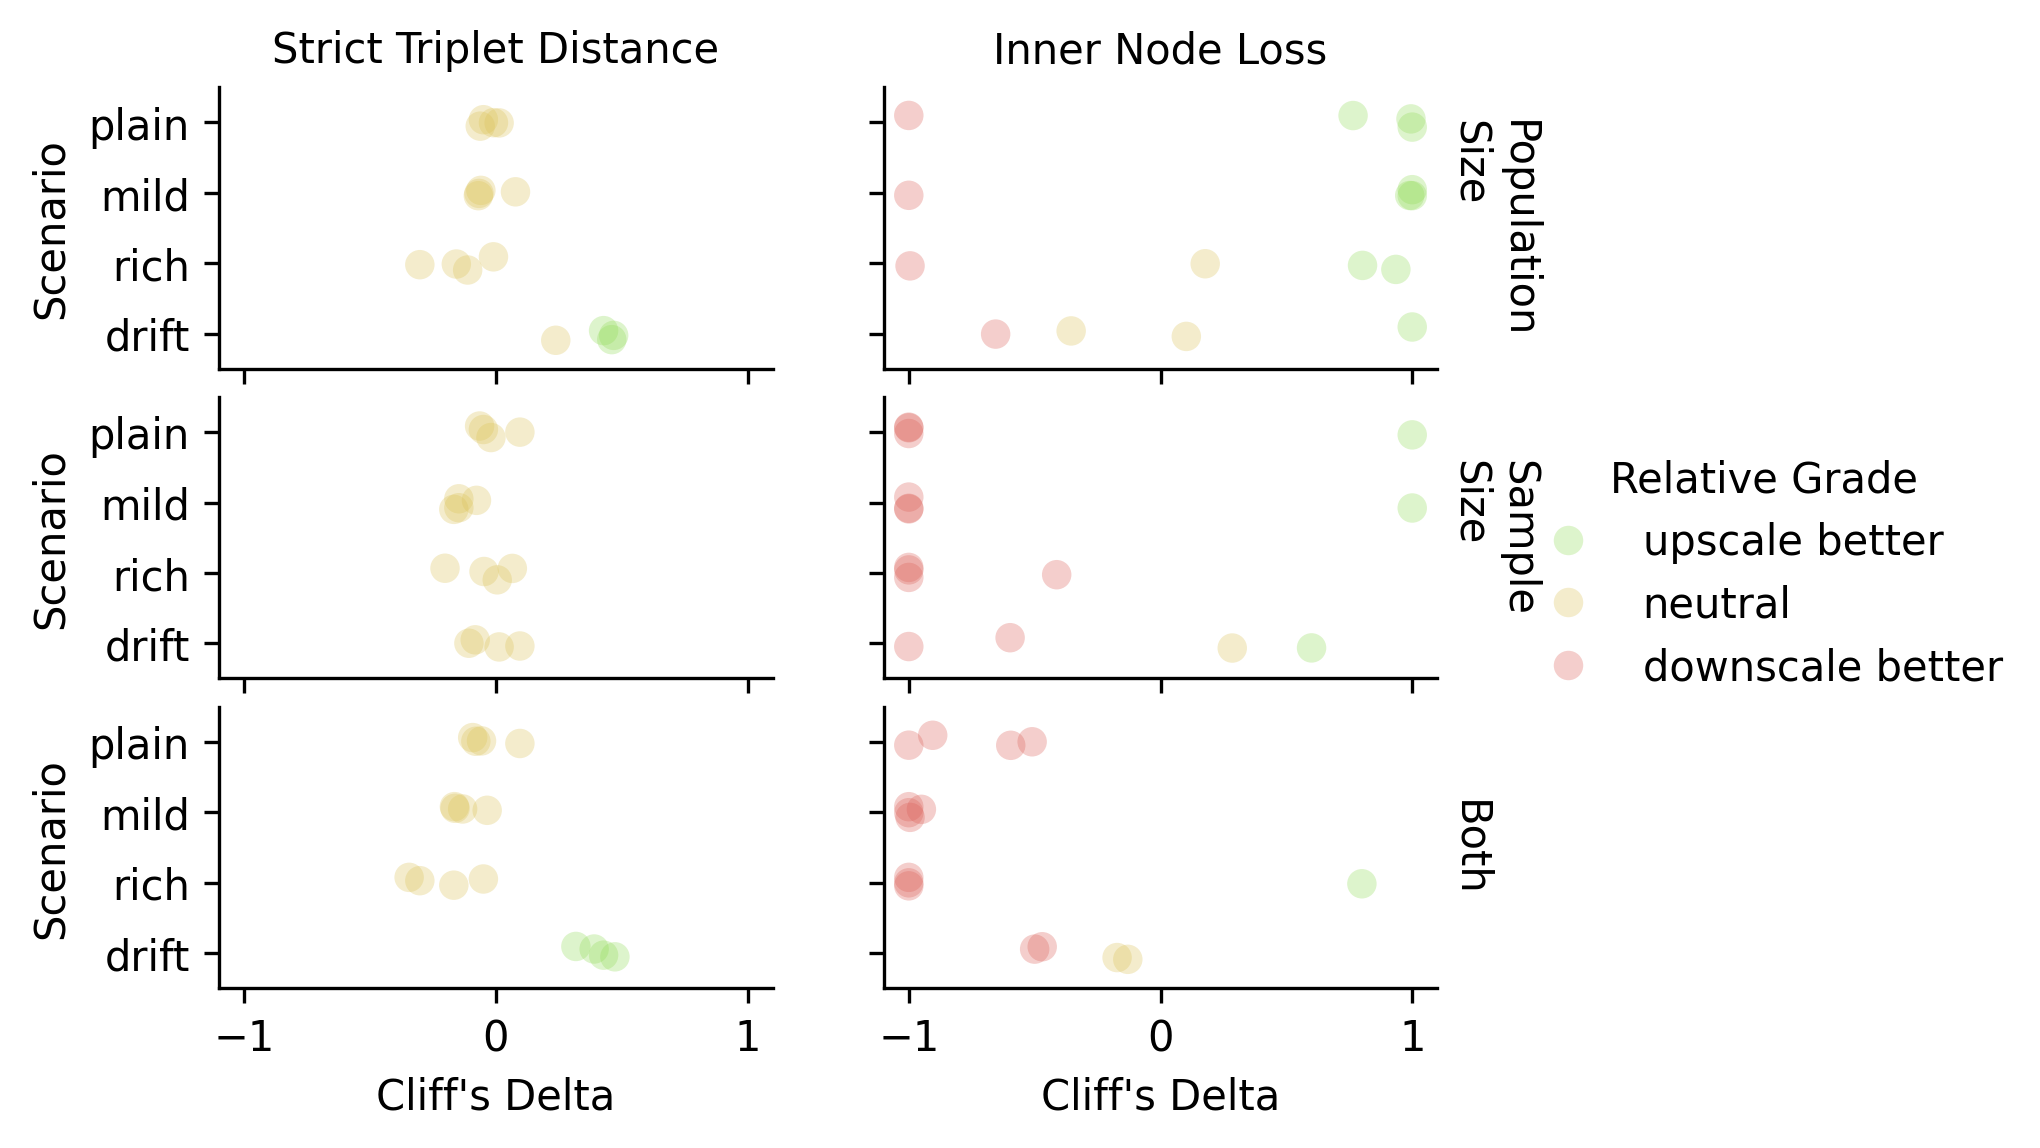
\includegraphics[height=1.7in,trim={2cm 0 5cm 0},clip]{binder/binder/dsamp-popsize-scale/teeplots/col=metric+hue=relative-grade+kind=strip+policy=hybrid+row=scaling-factor+viz=catplot+x=cliff-s-delta+y=scenario+ext=}
    \caption{hybrid retention policy (surface)}
  \end{subfigure}%
  \rulesep %
  \begin{subfigure}[b]{0.39\textwidth}
    \centering
    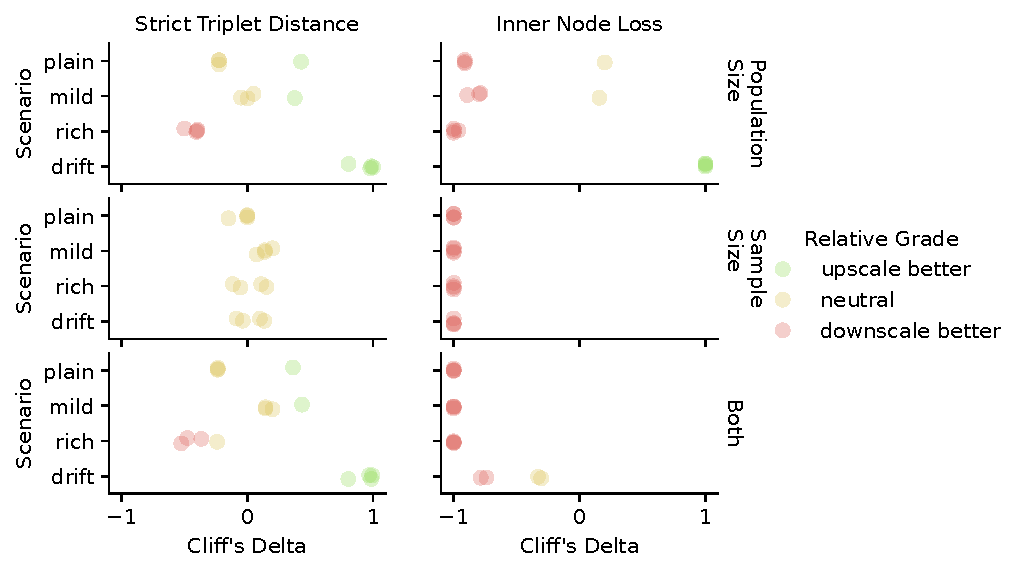
\includegraphics[height=1.7in,trim={2cm 0 0 0},clip]{binder/binder/dsamp-popsize-scale/teeplots/col=metric+hue=relative-grade+kind=strip+policy=steady+row=scaling-factor+viz=catplot+x=cliff-s-delta+y=scenario+ext=}
    \caption{steady retention policy (column)}
  \end{subfigure}
  \caption{%
  \textbf{How does scale impact reconstruction quality?}
  \footnotesize
  Each dot shows a Cliff's Delta effect size of downscale-vs-upscale comparison under one sensitivity analysis condition.
  Color coding indicates a significant outcome (Mann-Whitney U).
  In order, rows show scaling outcomes for increasing population size, population subsample size (i.e., tree tip count), and both these factors.
  For tilted and hybrid policies, scaling had minimal effects on triplet distance and no systematic effect on inner node loss.
  Inner node loss worsened when scaling sample size, with and without scaling population size.
  Scaling effects were more variable under steady retention policy.
  See Supplementary Figures \labelcref{fig:dsamp-popsize-scale-hybrid,fig:dsamp-popsize-scale-steady,fig:dsamp-popsize-scale-tilted} for listing of effects by sensitivity analysis condition \citep{moreno2024supplemental}.
  }
  \label{fig:scaling-summary}
\end{figure*}
